\documentclass[]{article}
\usepackage{lmodern}
\usepackage{amssymb,amsmath}
\usepackage{ifxetex,ifluatex}
\usepackage{fixltx2e} % provides \textsubscript
\ifnum 0\ifxetex 1\fi\ifluatex 1\fi=0 % if pdftex
  \usepackage[T1]{fontenc}
  \usepackage[utf8]{inputenc}
\else % if luatex or xelatex
  \ifxetex
    \usepackage{mathspec}
  \else
    \usepackage{fontspec}
  \fi
  \defaultfontfeatures{Ligatures=TeX,Scale=MatchLowercase}
\fi
% use upquote if available, for straight quotes in verbatim environments
\IfFileExists{upquote.sty}{\usepackage{upquote}}{}
% use microtype if available
\IfFileExists{microtype.sty}{%
\usepackage{microtype}
\UseMicrotypeSet[protrusion]{basicmath} % disable protrusion for tt fonts
}{}
\usepackage[margin=1in]{geometry}
\usepackage{hyperref}
\hypersetup{unicode=true,
            pdftitle={Assignment 2},
            pdfauthor={Per Emil Hammarlund, Albert Öst},
            pdfborder={0 0 0},
            breaklinks=true}
\urlstyle{same}  % don't use monospace font for urls
\usepackage{graphicx,grffile}
\makeatletter
\def\maxwidth{\ifdim\Gin@nat@width>\linewidth\linewidth\else\Gin@nat@width\fi}
\def\maxheight{\ifdim\Gin@nat@height>\textheight\textheight\else\Gin@nat@height\fi}
\makeatother
% Scale images if necessary, so that they will not overflow the page
% margins by default, and it is still possible to overwrite the defaults
% using explicit options in \includegraphics[width, height, ...]{}
\setkeys{Gin}{width=\maxwidth,height=\maxheight,keepaspectratio}
\IfFileExists{parskip.sty}{%
\usepackage{parskip}
}{% else
\setlength{\parindent}{0pt}
\setlength{\parskip}{6pt plus 2pt minus 1pt}
}
\setlength{\emergencystretch}{3em}  % prevent overfull lines
\providecommand{\tightlist}{%
  \setlength{\itemsep}{0pt}\setlength{\parskip}{0pt}}
\setcounter{secnumdepth}{0}
% Redefines (sub)paragraphs to behave more like sections
\ifx\paragraph\undefined\else
\let\oldparagraph\paragraph
\renewcommand{\paragraph}[1]{\oldparagraph{#1}\mbox{}}
\fi
\ifx\subparagraph\undefined\else
\let\oldsubparagraph\subparagraph
\renewcommand{\subparagraph}[1]{\oldsubparagraph{#1}\mbox{}}
\fi

%%% Use protect on footnotes to avoid problems with footnotes in titles
\let\rmarkdownfootnote\footnote%
\def\footnote{\protect\rmarkdownfootnote}

%%% Change title format to be more compact
\usepackage{titling}

% Create subtitle command for use in maketitle
\newcommand{\subtitle}[1]{
  \posttitle{
    \begin{center}\large#1\end{center}
    }
}

\setlength{\droptitle}{-2em}

  \title{Assignment 2}
    \pretitle{\vspace{\droptitle}\centering\huge}
  \posttitle{\par}
    \author{Per Emil Hammarlund, Albert Öst}
    \preauthor{\centering\large\emph}
  \postauthor{\par}
      \predate{\centering\large\emph}
  \postdate{\par}
    \date{2019-04-26}

\usepackage{float}
\let\origfigure\figure
\let\endorigfigure\endfigure
\renewenvironment{figure}[1][2] {
    \expandafter\origfigure\expandafter[H]
} {
    \endorigfigure
}

\begin{document}
\maketitle

\section{Visualization of the sound
files}\label{visualization-of-the-sound-files}

Figure 1 shows the momentary amplitude over time for each of the two
audio files.

\begin{figure}
\centering
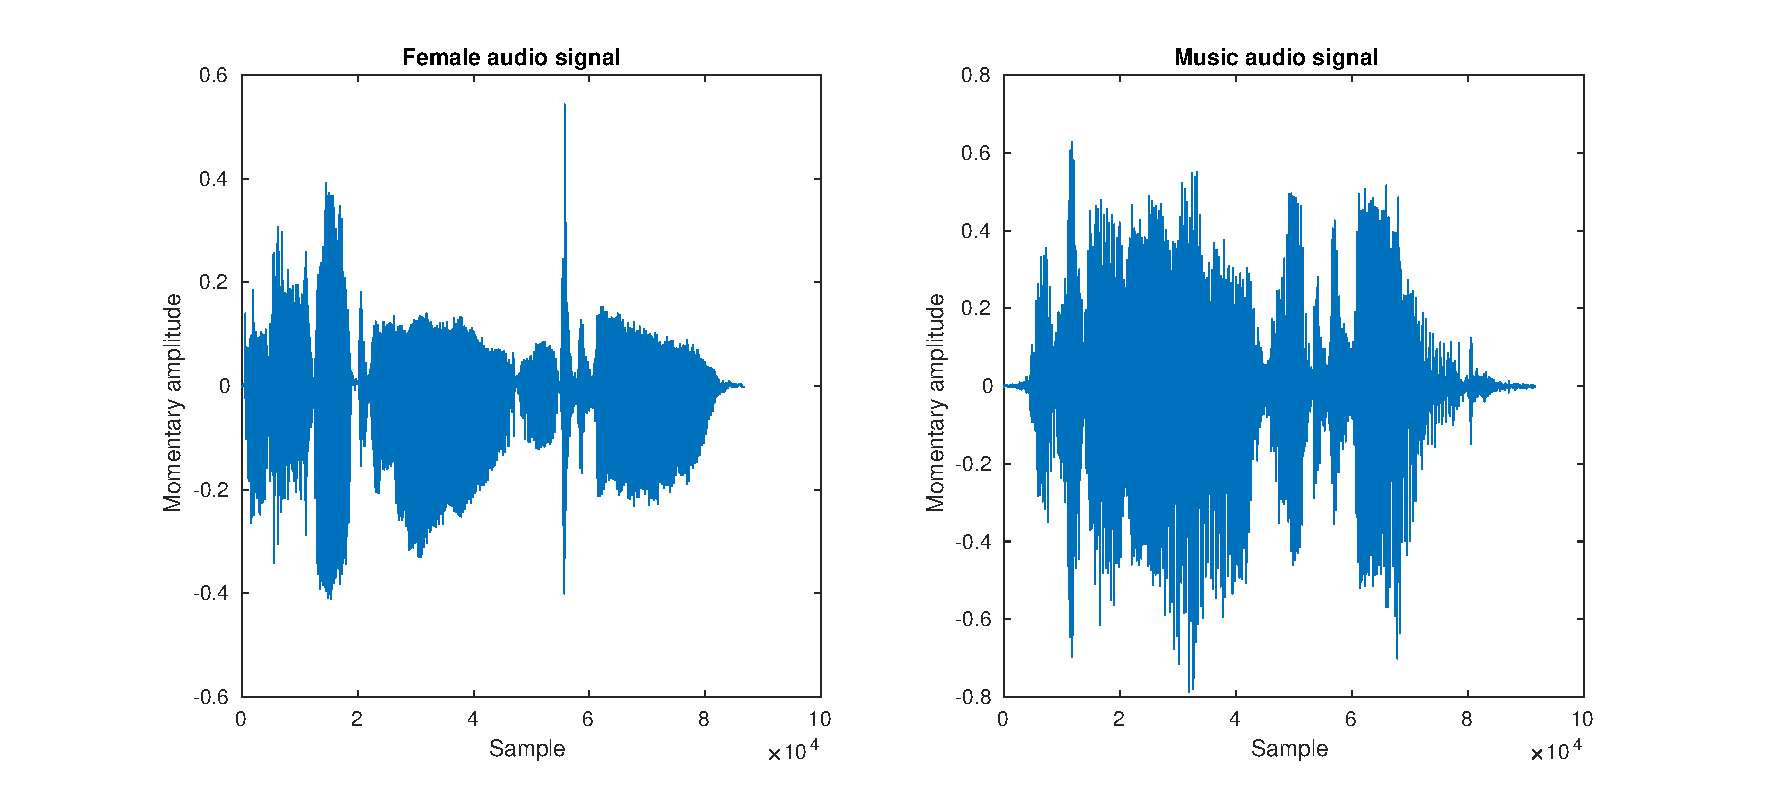
\includegraphics{Result_Pics/female_music_waveform.eps}
\caption{Momentary amplitude over time}
\end{figure}

Next, we zoomed in on a range of 20 milliseconds, this corresponded to
\(44100 * 20 \cdot 10^{-3}\) samples. This gave the following
observation:

\begin{figure}
\centering
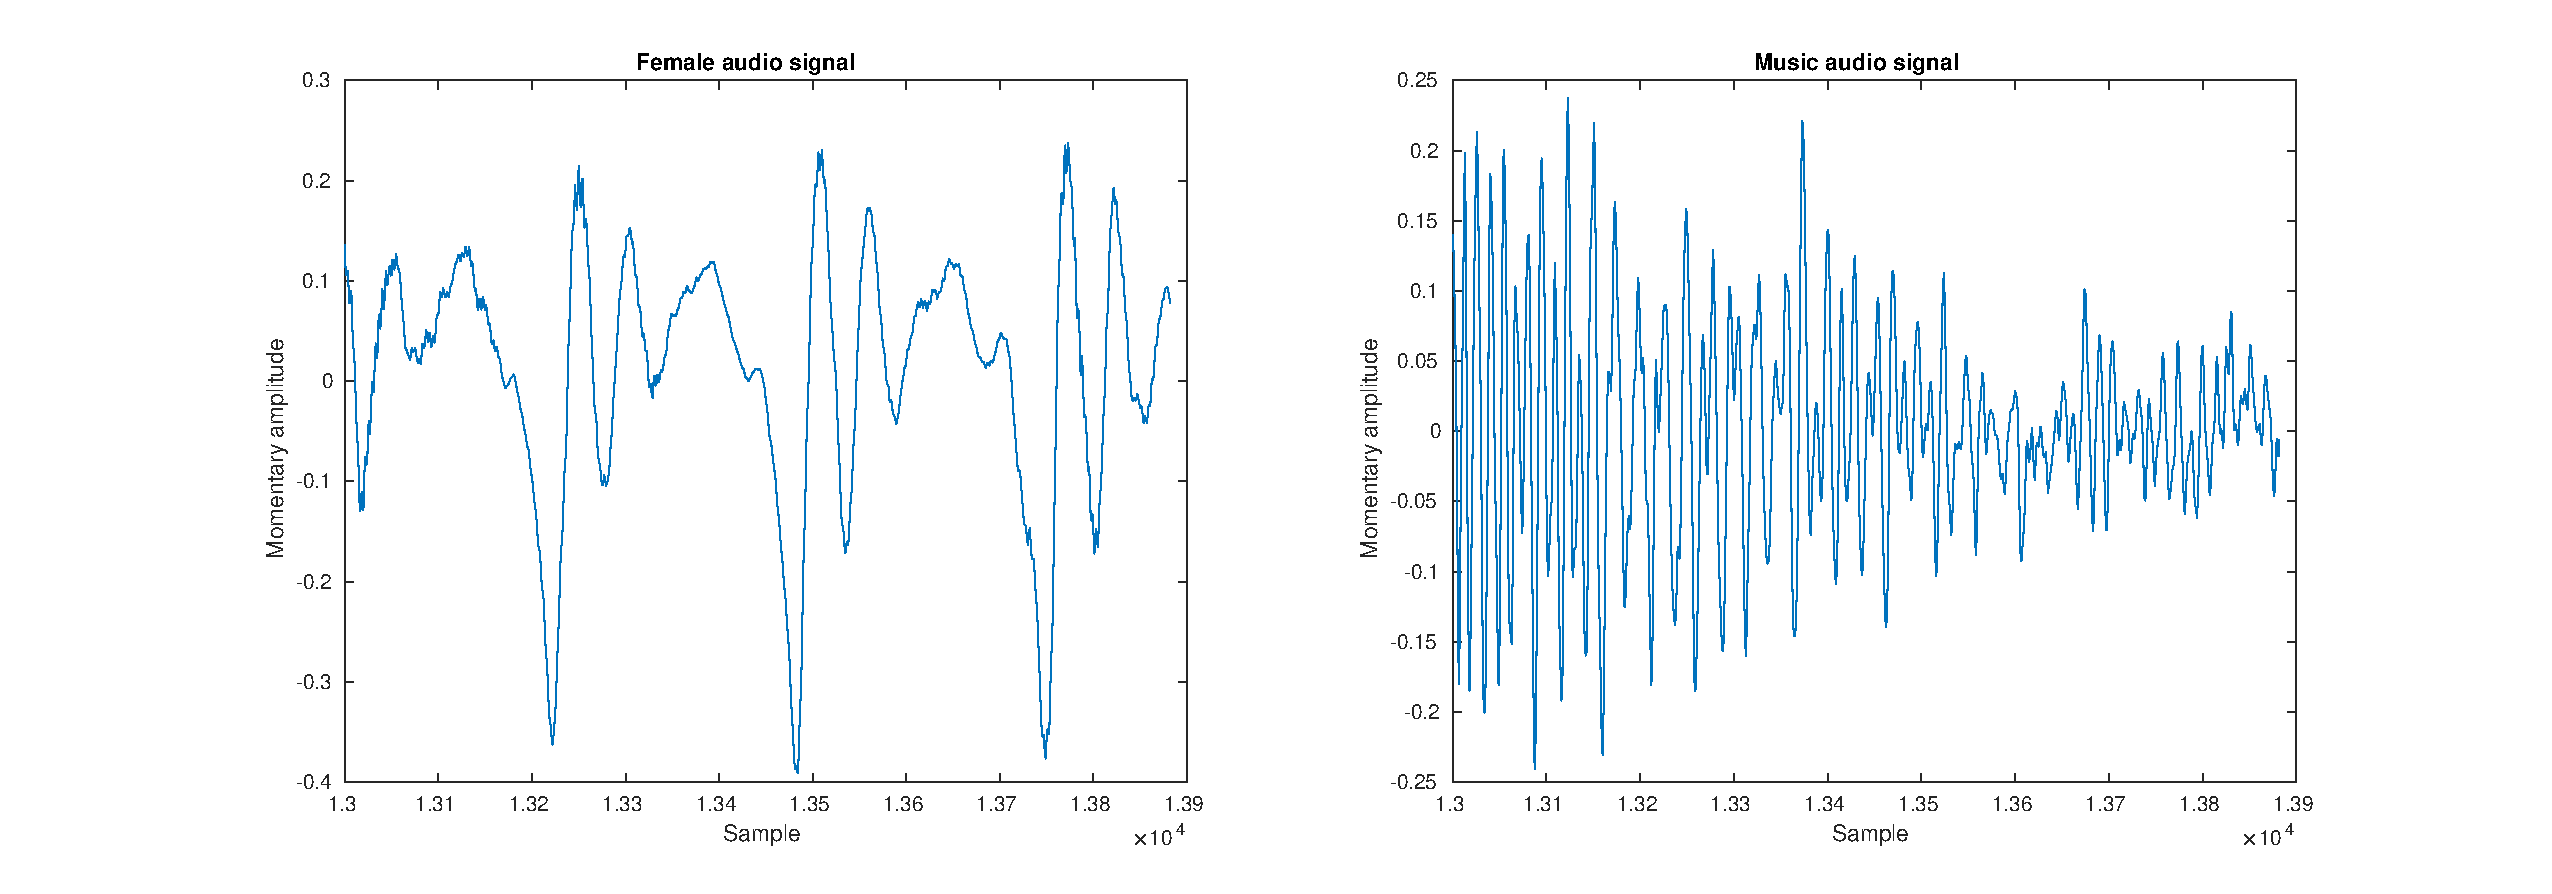
\includegraphics{Result_Pics/female_music_waveform_20ms.eps}
\caption{Momentary amplitude in 20ms timeframe}
\end{figure}

As can be seen in in figure 2 above, the behavior of the sound signal
from the two audio files has an oscillatory behavior.

\newpage

\section{Voiced and unvoiced speech
segments}\label{voiced-and-unvoiced-speech-segments}

Figure 3 below shows a plot of the momentary amplitude for the ``sh''
sound from the female voice audio file.

\begin{figure}
\centering
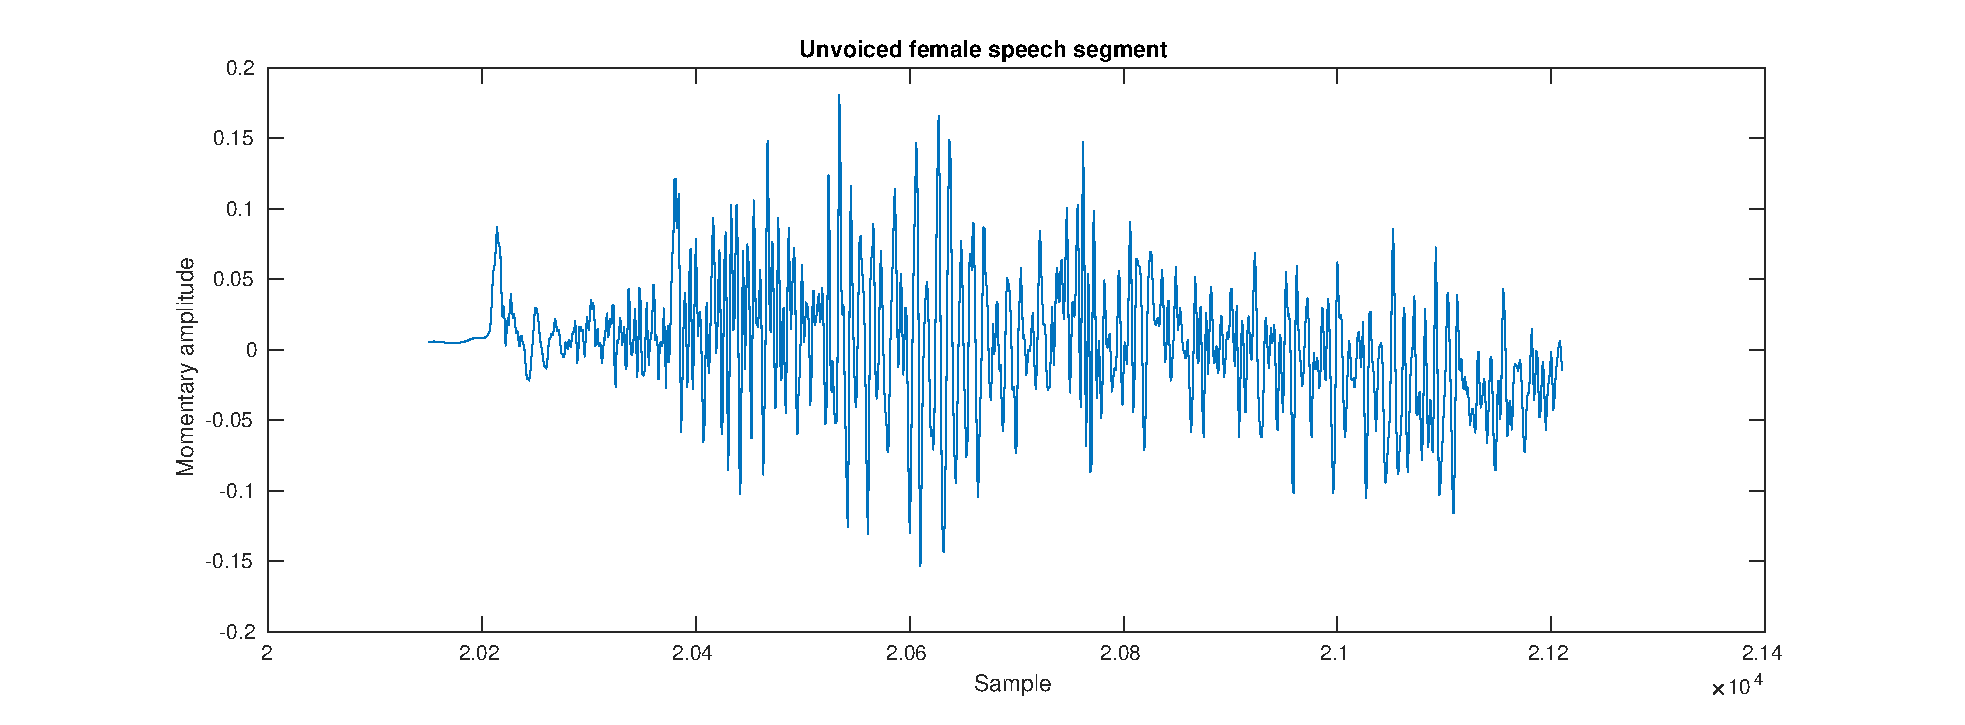
\includegraphics{Result_Pics/female_music_waveform_unvoiced_segment.eps}
\caption{Visualization of unvoiced segment from female voice sound file}
\end{figure}

As can be seen in figure 3, the unvoiced signal is not harmonic and
looks more like random noise.

Figure 4 shows a plot of the momentary amplitude of the voiced ``O''
sound.

\begin{figure}
\centering
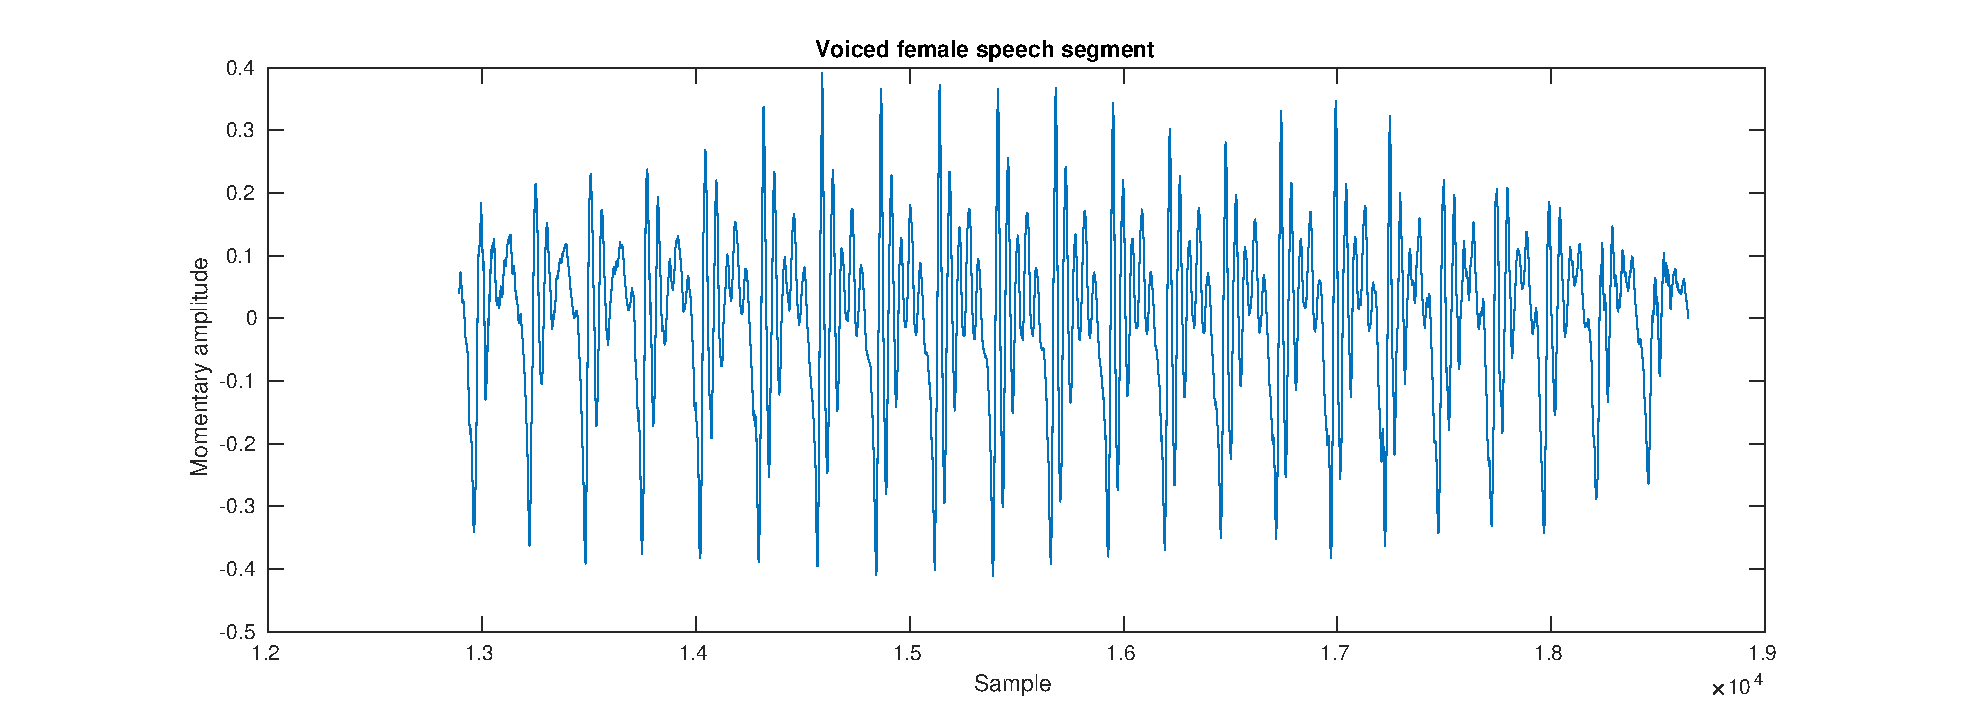
\includegraphics{Result_Pics/female_music_waveform_voiced_segment.eps}
\caption{Visualization of voiced speech segment from female voice sound
file}
\end{figure}

From figure 4, we can see that the voiced sound has a harmonic behavior
and follows a distinct pattern.

\newpage

\section{Spectrogram of sound files}\label{spectrogram-of-sound-files}

Figure 5 points out the unvoiced and voiced segments of the female voice
file and shows the harmonics of the music file.

\begin{figure}
\centering
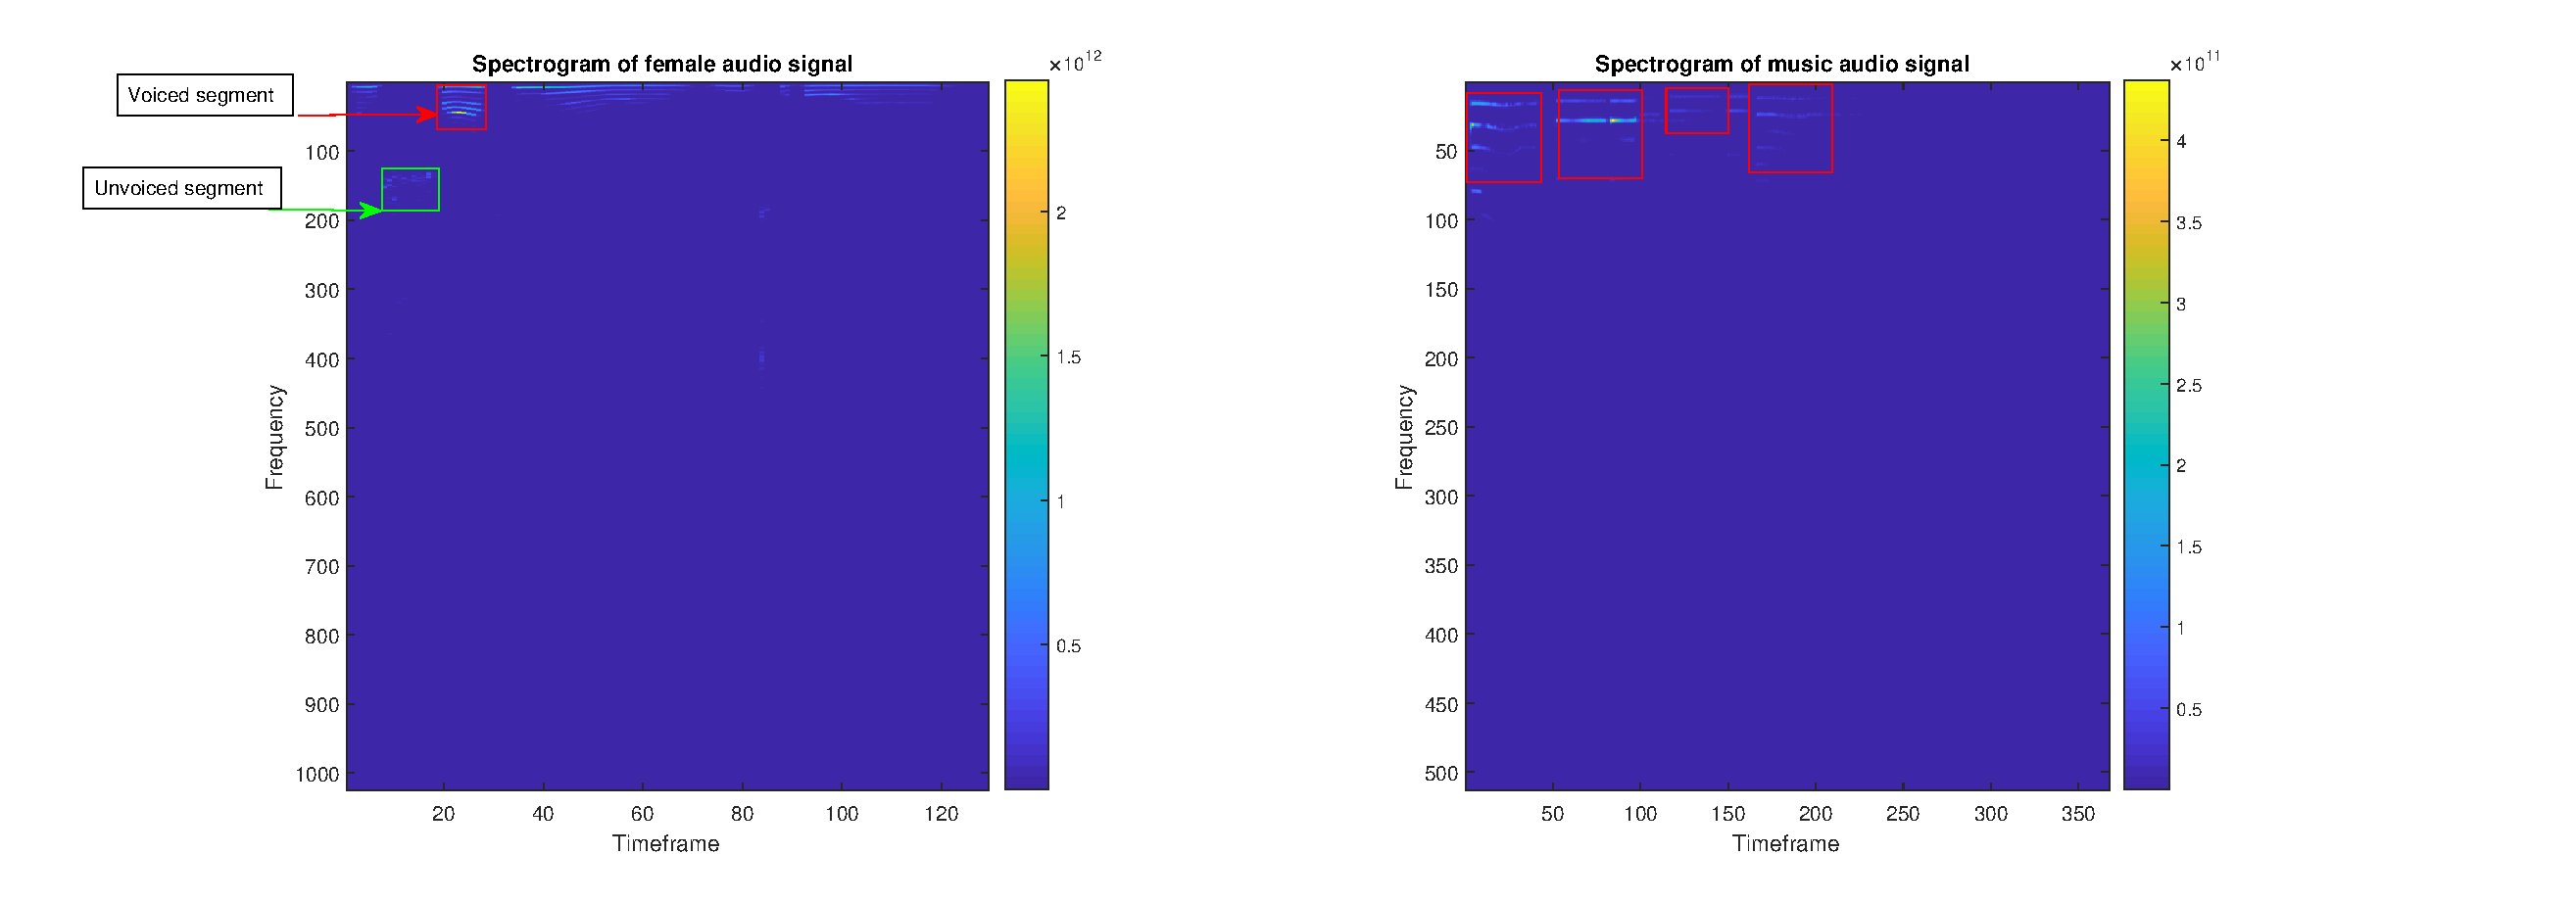
\includegraphics{Result_Pics/female_music_spetgram_marked.eps}
\caption{Annotated spectrogram of audio files}
\end{figure}

In the two spectrograms, the red boxes point out audio segments with
harmonic behavior.

Figure 6 shows the logged version of the spectrograms:

\begin{figure}
\centering
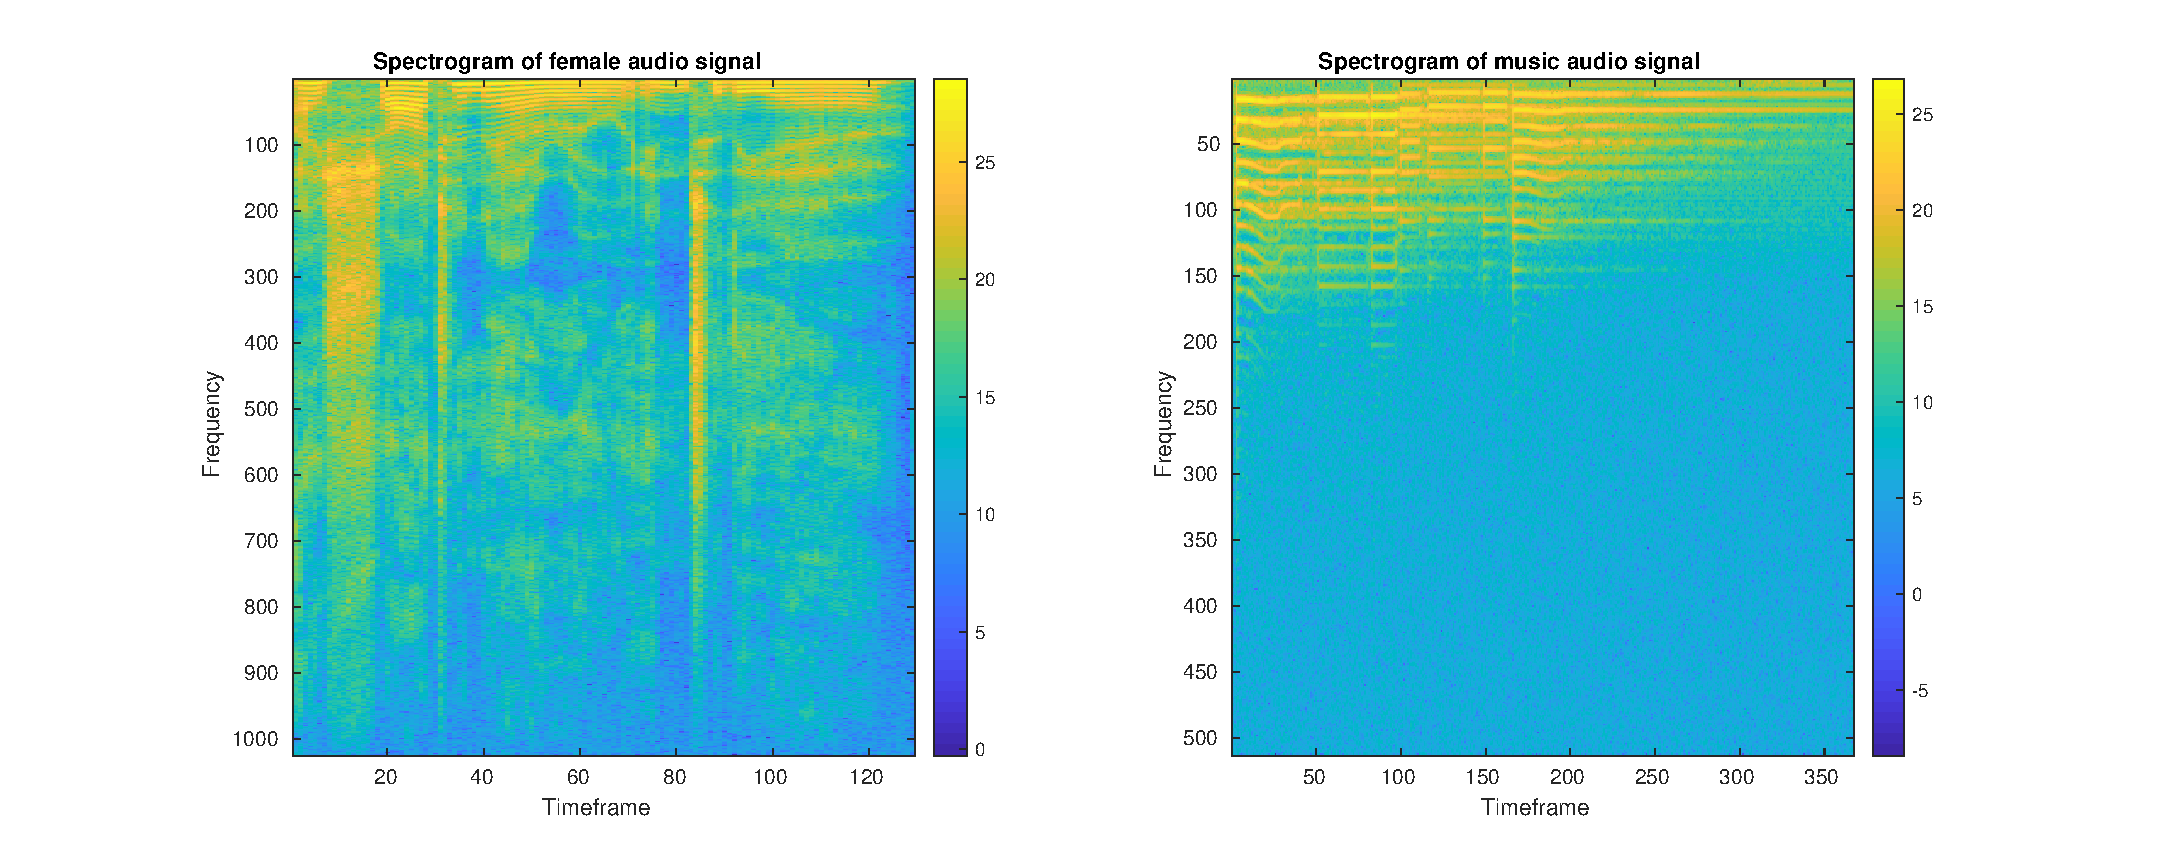
\includegraphics{Result_Pics/female_music_spetgram_log.eps}
\caption{Logged version of the spectrograms for the two audio files}
\end{figure}

\newpage

\section{Comparison between ceptrogram and
spectrogram}\label{comparison-between-ceptrogram-and-spectrogram}

Figure 7 and 8 show comparisons between the spectrogram and ceptrogram
representation of the audio files:

\begin{figure}
\centering
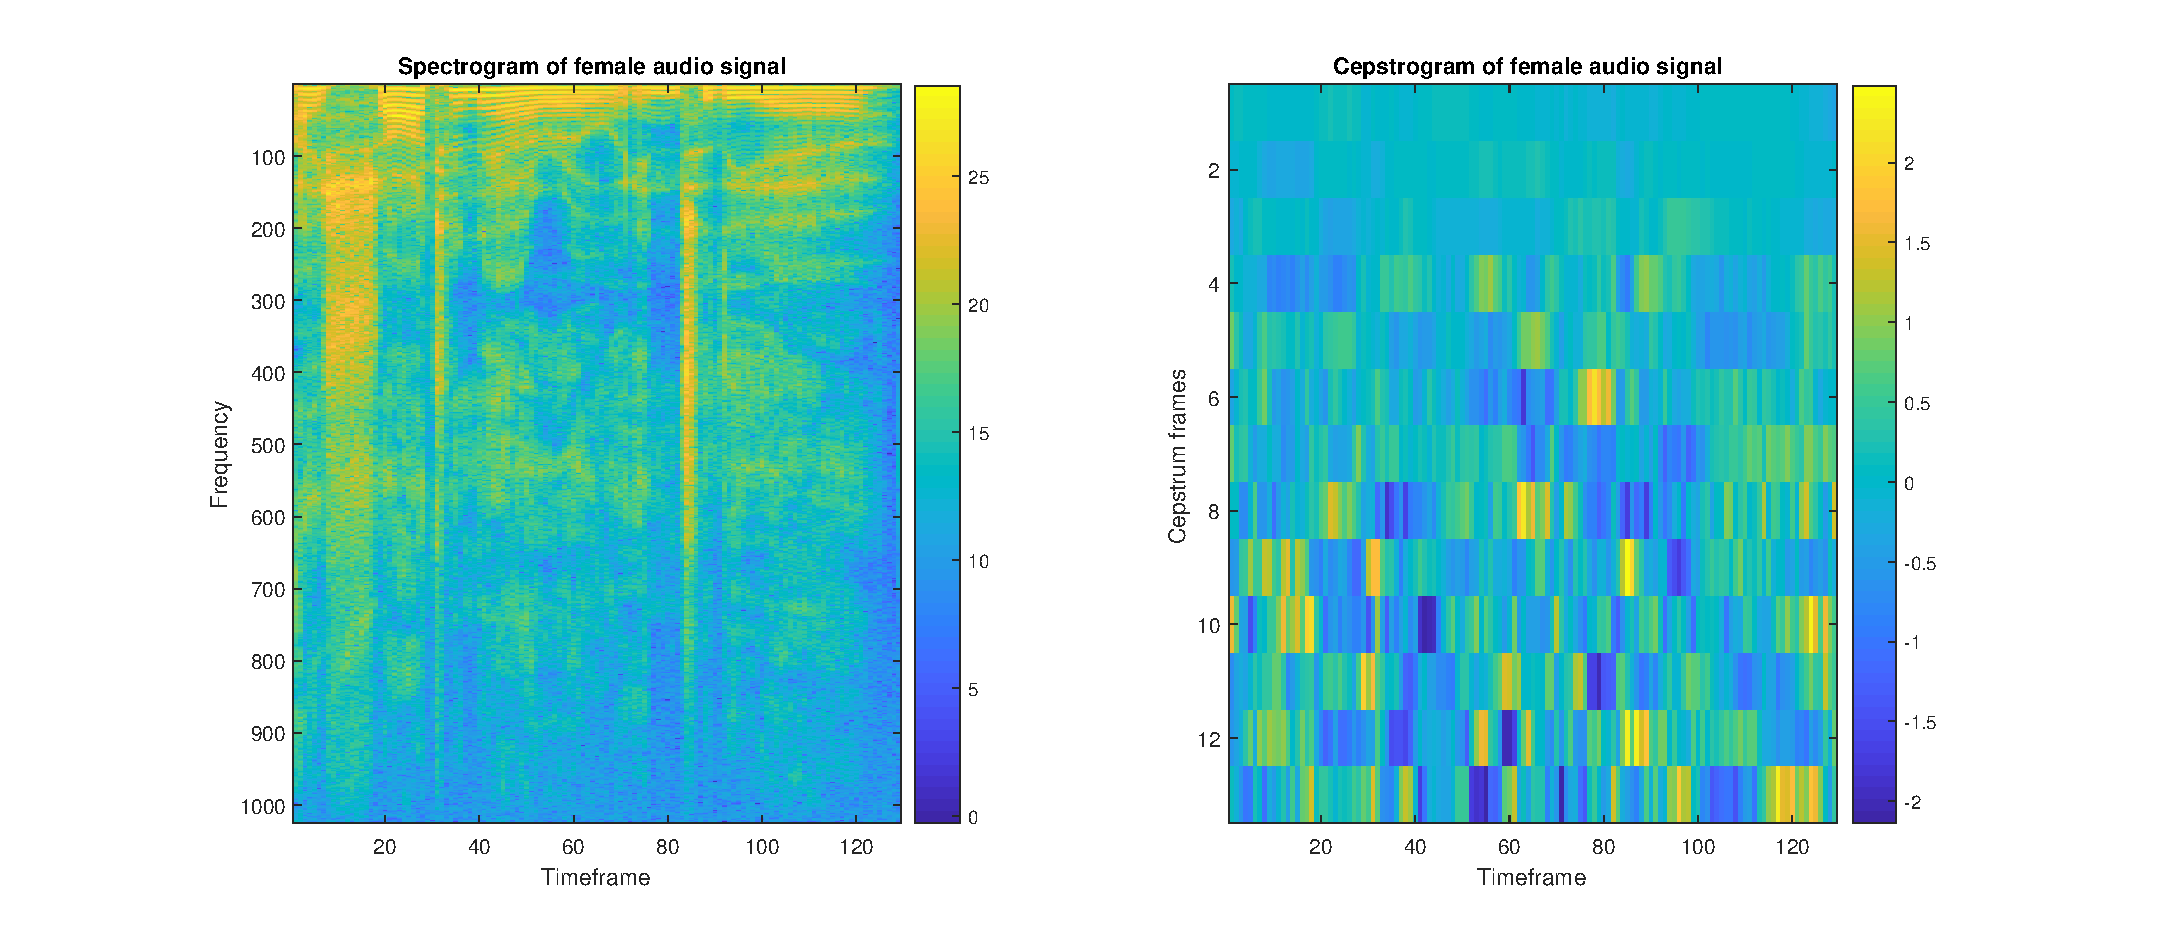
\includegraphics{Result_Pics/spetgram_cepgram_female.eps}
\caption{Spectrogram and ceptrogram representation of the female audio
file}
\end{figure}

\begin{figure}
\centering
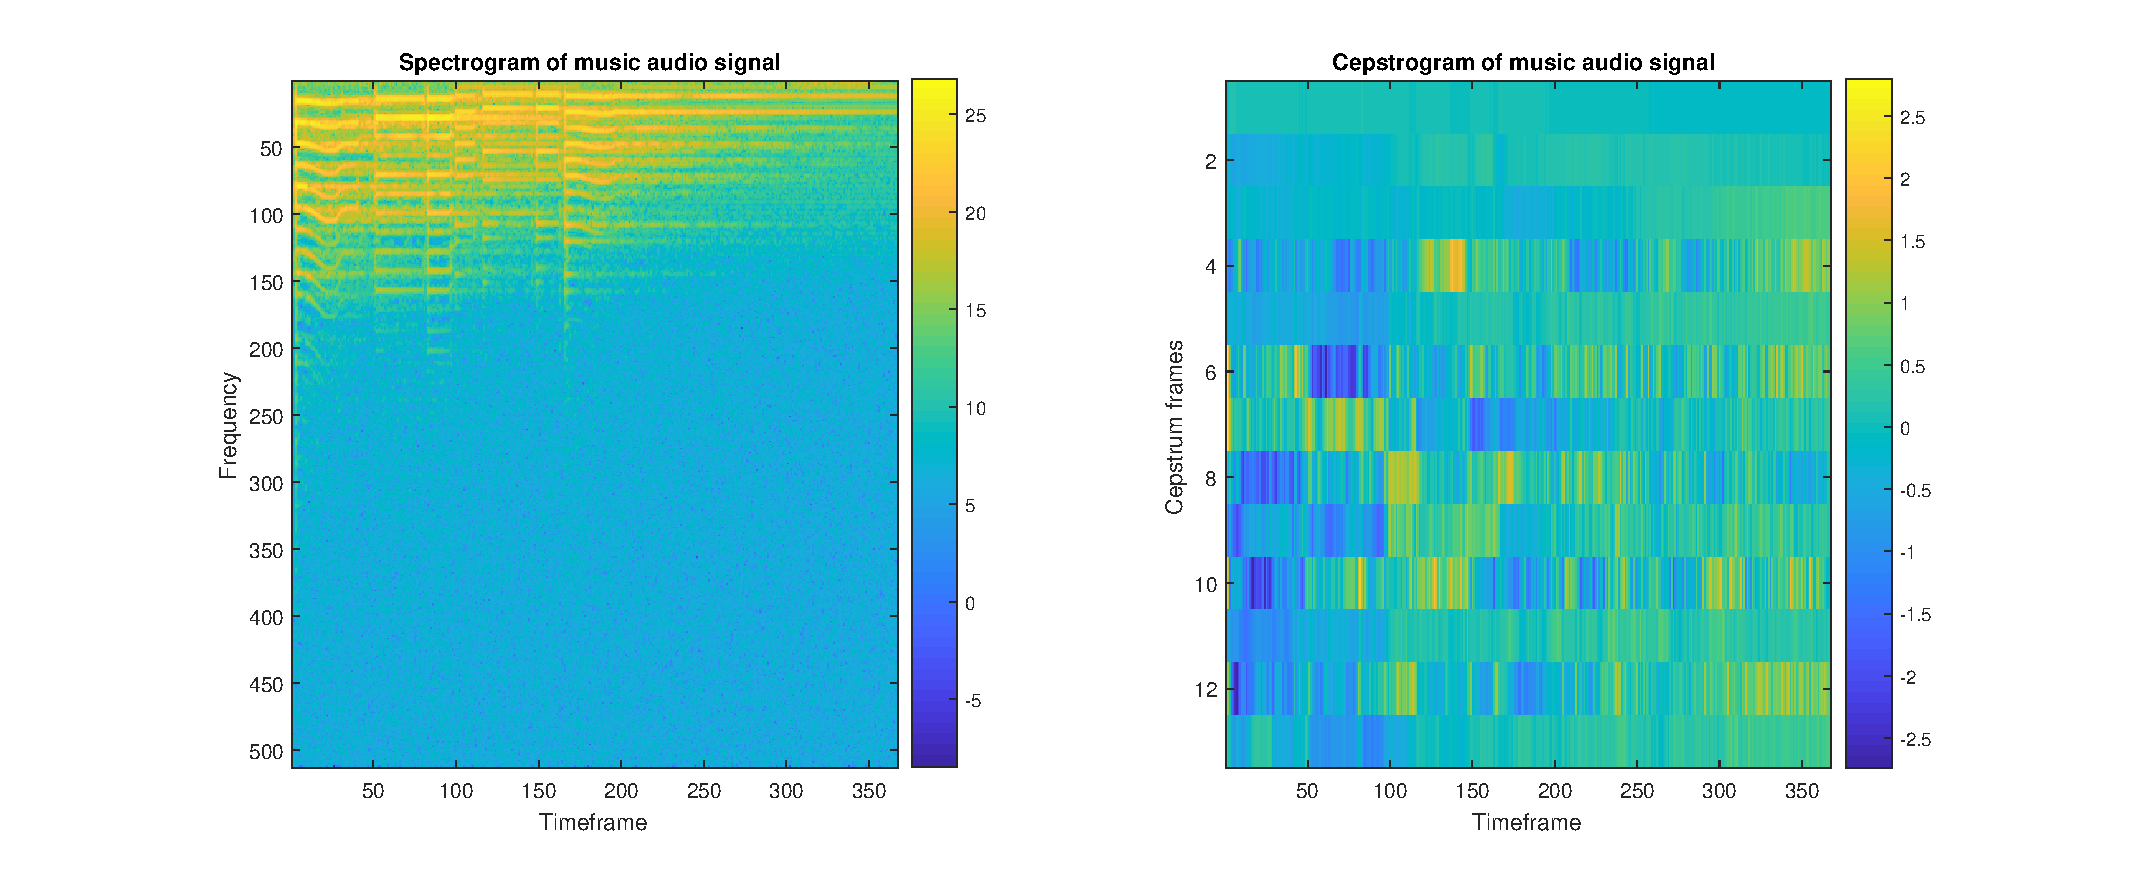
\includegraphics{Result_Pics/spetgram_cepgram_music.eps}
\caption{Spectrogram and ceptrogram representation of the music audio
file}
\end{figure}

When comparing the two representation in the visualization of the female
voice. Voiced and unvoiced segments are easily identifiable in
spectrogram, and hard to identify as a human being in the ceptrogram.
However, it is easier to see the intensity of each band pass (cepstrum
frame) in the cepstrogram.

\newpage

\section{Comparison between male and female
audio}\label{comparison-between-male-and-female-audio}

Figure 9 shows the spectrogram for the female and male audio signals.

\begin{figure}
\centering
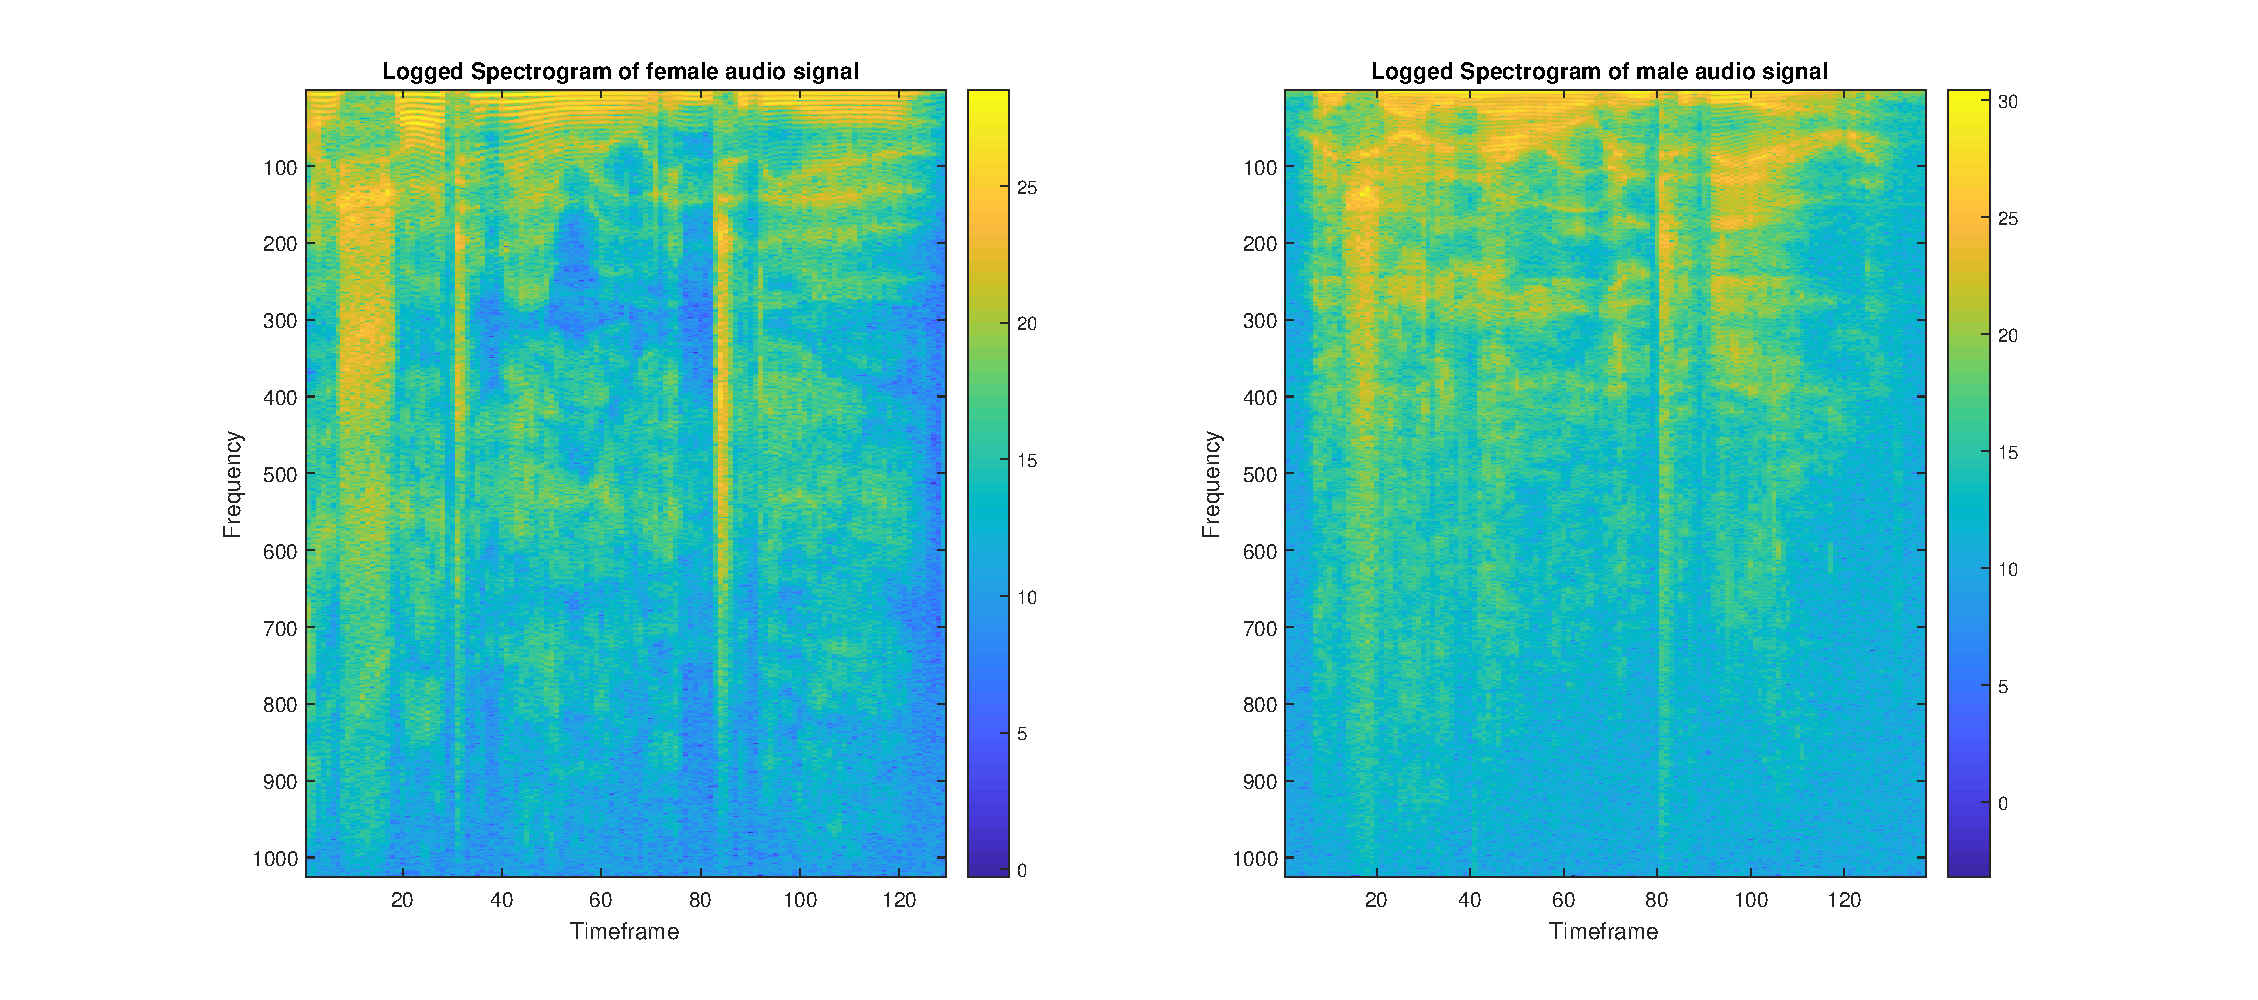
\includegraphics{Result_Pics/female_male_spetgram.eps}
\caption{Spectrograms of female and male audio signals}
\end{figure}

Looking at figure 9, it is visible that the female and male audio
signals have roughly the same form. However, this would be hard for a
computer to see due to the high complexity of comparing the two signals.

Figure 10 shows a comparison between the male and female audio files.

\begin{figure}
\centering
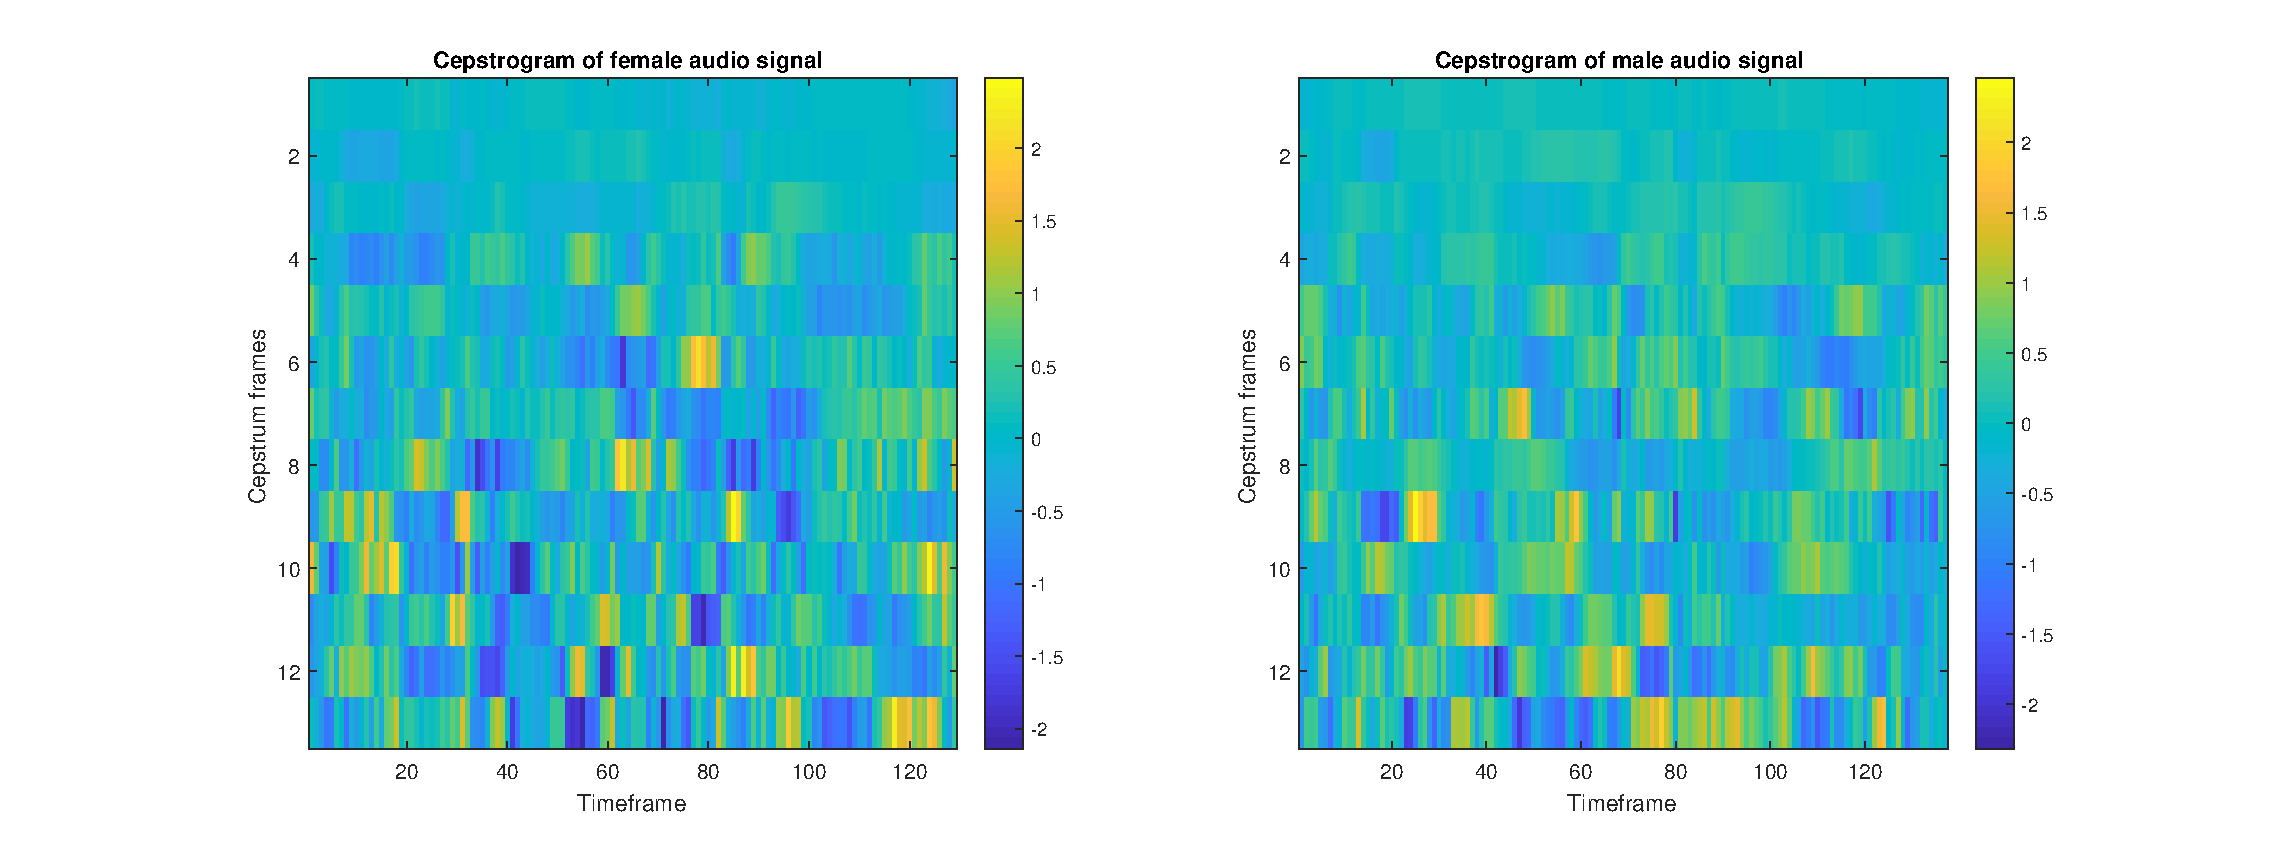
\includegraphics{Result_Pics/cepgram_male_female.eps}
\caption{Cepstrograms of male and female audio signals}
\end{figure}

As can be seen in figure 10 above, the cepstrograms of the female and
male audio files roughly have the same intensity at the same points.
This make sense since cepstrograms are supposed to be pitch invariant.
This would be far easier for a computer to infer as well due to the
decreased dimensionality of the representation of the audio signals.

Figure 11 and 12 below show the correlation matrices between the male
and female audio files.

\begin{figure}
\centering
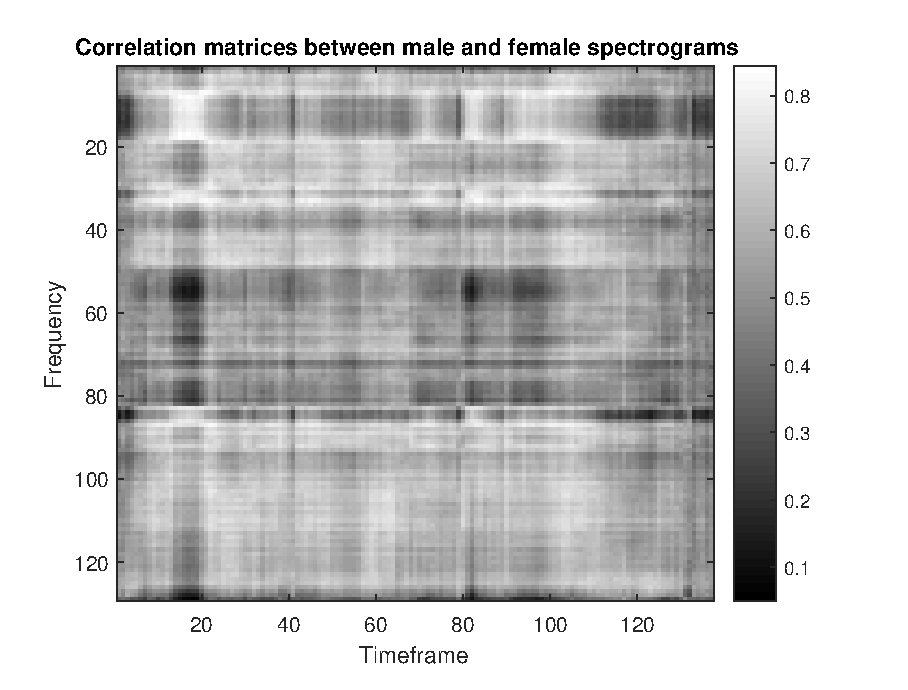
\includegraphics{Result_Pics/corr_female_male_spetgram.eps}
\caption{Correlation between male and female spectrograms}
\end{figure}

\begin{figure}
\centering
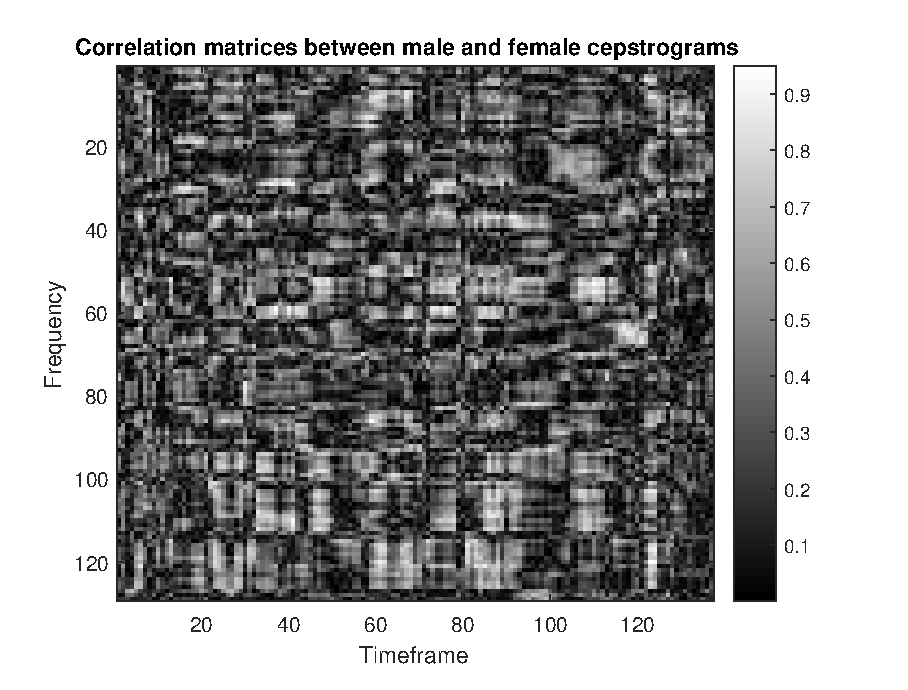
\includegraphics{Result_Pics/corr_female_male_cepgram.eps}
\caption{Correlation between male and female cepstrograms}
\end{figure}

From which it can be seen that the spectrograms are more correlated. The
correlation between the cepstrograms of the male and female audio is far
smaller and is therefore the more diagonal of the two.

\newpage

\section{Extraction of dynamic
features}\label{extraction-of-dynamic-features}

The dynamic features where extracted by writing the following ocde (see
assignment2.m for original source):

\begin{verbatim}
% Extraction of dynamic features
dyn_female_cepgram = zeros(ncep * 3, size(female_mfccs, 2));
dyn_female_cepgram(1:ncep, :) = female_mfccs;
dyn_female_cepgram(ncep + 1 : 2 * ncep, 1) = zeros(ncep, 1);
dyn_female_cepgram(ncep + 1: 2 * ncep, 2:end) = diff(female_mfccs, 1, 2);
dyn_female_cepgram(2 * ncep + 1: end, 1) = zeros(ncep, 1);
dyn_female_cepgram(2 * ncep + 1 : end, 3:end) = diff(female_mfccs, 2, 2);

dyn_male_cepgram = zeros(ncep * 3, size(male_mfccs, 2));
dyn_male_cepgram(1:ncep, :) = male_mfccs;
dyn_male_cepgram(ncep + 1 : 2 * ncep, 1) = zeros(ncep, 1);
dyn_male_cepgram(ncep + 1: 2 * ncep, 2:end) = diff(male_mfccs, 1, 2);
dyn_male_cepgram(2 * ncep + 1: end, 1) = zeros(ncep, 1);
dyn_male_cepgram(2 * ncep + 1 : end, 3:end) = diff(male_mfccs, 2, 2);
\end{verbatim}

\newpage

\section{Some thoughts on the possibility of fooling the
MFCC}\label{some-thoughts-on-the-possibility-of-fooling-the-mfcc}

The sounds ``ch'' and ``sh'' are easily distinguishable from each other
for humans. But the MFCC will only see these as unvoiced utterances with
same spread. The same text with a strong dialect would be seen as a
different utterance in the feature extractor, but a human listenser with
a keen ear would have little trouble understanding. Humans also have the
ability to filter out ambient noise (such as a load crowd) and hear what
is being said. The feature extractor on the other hand, will be unable
to filter out to the desired source.

Since the MFCC feature extractor removes information, it will not be
able to find differences that can not be found in the original sound.


\end{document}
